Following the approach in the earlier problems, it is obvious that
	\begin{align}
		\vec{n} 
			= \vec{e}_2,
	\vec{c} =\vec{u}=\vec{0}.
\end{align}
Consequently,
%
\begin{align}
	\vec{V} &= \myvec{1 &0\\ 0 & 1-e^2}
	\\
	\vec{F} &= ce^2\vec{e}_2 \implies \norm{\vec{F}} = ce^2=5
\label{eq:chapters/11/11/4/9/F}
	\\
	f 
	  &= 25 - c^2 e^2
\label{eq:chapters/11/11/4/9/f}
\end{align}
%
Since the vertices are  on the conic,
\begin{align}
	\vec{v_1}^{\top}\vec{V}\vec{v_1} +2\vec{u}^{\top}\vec{v_1}+f &= 0\\
\implies 9\brak{1-e^2} + f &= 0\\
 \label{eq:chapters/11/11/4/9/1}
\end{align}
Solving \eqref{eq:chapters/11/11/4/9/1},
\eqref{eq:chapters/11/11/4/9/F}
and
\eqref{eq:chapters/11/11/4/9/f},
\begin{align}
	c = \frac{9}{5},\ 
	e = \frac{5}{3},
\end{align}
%
yielding
\begin{align}
	\vec{V} = \myvec{1&0\\0& -\frac{16}{9}} ,\
	\vec{u} = \myvec{0\\0},\
	f = 16.
\end{align}
%
Thus, the desired equation of the hyperbola is
\begin{align}
	\vec{x}^{\top} \myvec{1&0\\ 0 & -\frac{16}{9}} \vec{x} +16 =0
\end{align}
%
See
%
    \figref{fig:chapters/11/11/4/9/}.
\begin{figure}[h!]
  \centering
    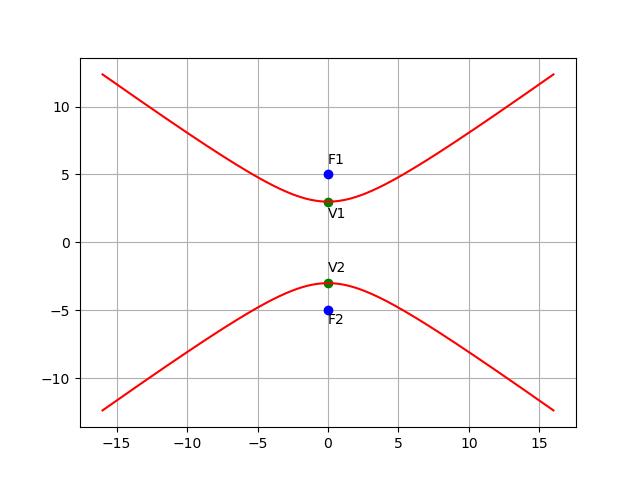
\includegraphics[width=\columnwidth]{chapters/11/11/4/9/figs/Figure_1.png}
    \caption{Figure 1}
    \label{fig:chapters/11/11/4/9/}
\end{figure}
%



